% Template for ICASSP-2021 paper; to be used with:
%          spconf.sty  - ICASSP/ICIP LaTeX style file, and
%          IEEEbib.bst - IEEE bibliography style file.
% --------------------------------------------------------------------------
\documentclass{article}
\usepackage{spconf,amsmath, amssymb}
\usepackage{xcolor, graphicx}
\usepackage{mathtools} % for constraints matrix
% Example definitions.
% --------------------
\def\x{{\mathbf x}}
\def\L{{\cal L}}

% signal vectors
\def\R{\mathbb{R}} %Real Numbers
\newcommand{\fP}{\vec{f}_P }
\newcommand{\fC}{\vec{f}_C }
\newcommand{\fH}{\vec{f}_H }
\newcommand{\fN}{\vec{f}_N }
\newcommand{\sP}{\vec{s}_P }
\newcommand{\sC}{\vec{s}_C }
\newcommand{\sH}{\vec{s}_H }
\newcommand{\sN}{\vec{s}_N }
\newcommand{\zP}{\vec{z}_P }
\newcommand{\zC}{\vec{z}_C }
\newcommand{\zH}{\vec{z}_H }
\newcommand{\zN}{\vec{z}_N }
\newcommand{\yP}{\vec{y}_P }
\newcommand{\yC}{\vec{y}_C }
\newcommand{\yH}{\vec{y}_H }
\newcommand{\yN}{\vec{y}_N }

% Title.
% ------
\title{AUTHOR GUIDELINES FOR ICASSP 2021 PROCEEDINGS MANUSCRIPTS}
%
% Single address.
% ---------------
\name{Jocelyn Ornelas Mu\~{n}oz$^{\star}$, Erica Rutter$^{\star}$ , Mario Ba\~{n}uelos$^{\dagger}$ , Roummel F. Marcia$^{\star}$}
%\name{Author(s) Name(s)\thanks{Thanks to XYZ agency for funding.}}
\address{$^{\star}$ Department of Applied Mathematics University of California, Merced \\
	$^{\dagger}$Department of Mathematics California State University, Fresno}

%

% For example:
% ------------
%\address{School\\
	%	Department\\
	%	Address}
%
% Two addresses (uncomment and modify for two-address case).
% ----------------------------------------------------------
%\twoauthors
%  {A. Author-one, B. Author-two\sthanks{Thanks to XYZ agency for funding.}}
%	{School A-B\\
	%	Department A-B\\
	%	Address A-B}
%  {C. Author-three, D. Author-four\sthanks{The fourth author performed the work
		%	while at ...}}
%	{School C-D\\
	%	Department C-D\\
	%	Address C-D}
%
\begin{document}
	\ninept
	%
	\maketitle
	%
	\begin{abstract}
%		The abstract should appear at the top of the left-hand column of text, about
%		0.5 inch (12 mm) below the title area and no more than 3.125 inches (80 mm) in
%		length.  Leave a 0.5 inch (12 mm) space between the end of the abstract and the
%		beginning of the main text.  The abstract should contain about 100 to 150
%		words, and should be identical to the abstract text submitted electronically
%		along with the paper cover sheet.  All manuscripts must be in English, printed
%		in black ink.
Structural variants (SVs) -- such as insertions, deletions, and duplications of an individual’s genome --represent an important class of genetic mutations which have been associated with both genetic diseases (e.g. cancer) and promotion of genetic diversity. Common approaches to detect SVs in an unknown genome require sequencing fragments of the genome, comparing them to a high-quality reference genome, and predicting SVs based on identified discordant fragments. However, inferring SVs from sequencing data has proven to be a challenging mathematical and computational problem because true SVs are rare and prone to low-coverage noise. We developed a computational method which seeks to improve existing SV detection methods in three ways: First, we generalize previous work by implementing an optimization approach consisting of a negative binomial log-likelihood objective function. Second, we use a block-coordinate descent approach to simultaneously predict if an SV is homozygous (SV is on two chromosomes) or heterozygous (SV is on one chromosome) given genomic data of related individuals. Third, we model a biologically realistic scenario where variants in the child are either inherited –and therefore must be present in the parent—or novel. We present results on simulated data, which demonstrate improvements in predicting SVs and uncovering true SVs from false positives. 
	\end{abstract}
	%
	\begin{keywords}
		One, two, three, four, five
	\end{keywords}
	%
	\section{INTRODUCTIONS}
	\label{sec:intro}
	
	These guidelines include complete descriptions of the fonts, spacing, and
	related information for producing your proceedings manuscripts. Please follow
	them and if you have any questions, direct them to Conference Management
	Services, Inc.: Phone +1-979-846-6800 or email
	to \\\texttt{papers@2021.ieeeicassp.org}.
	
	\begin{figure}[htb]
				\begin{minipage}[b]{1.0\linewidth}
						\centering
						\centerline{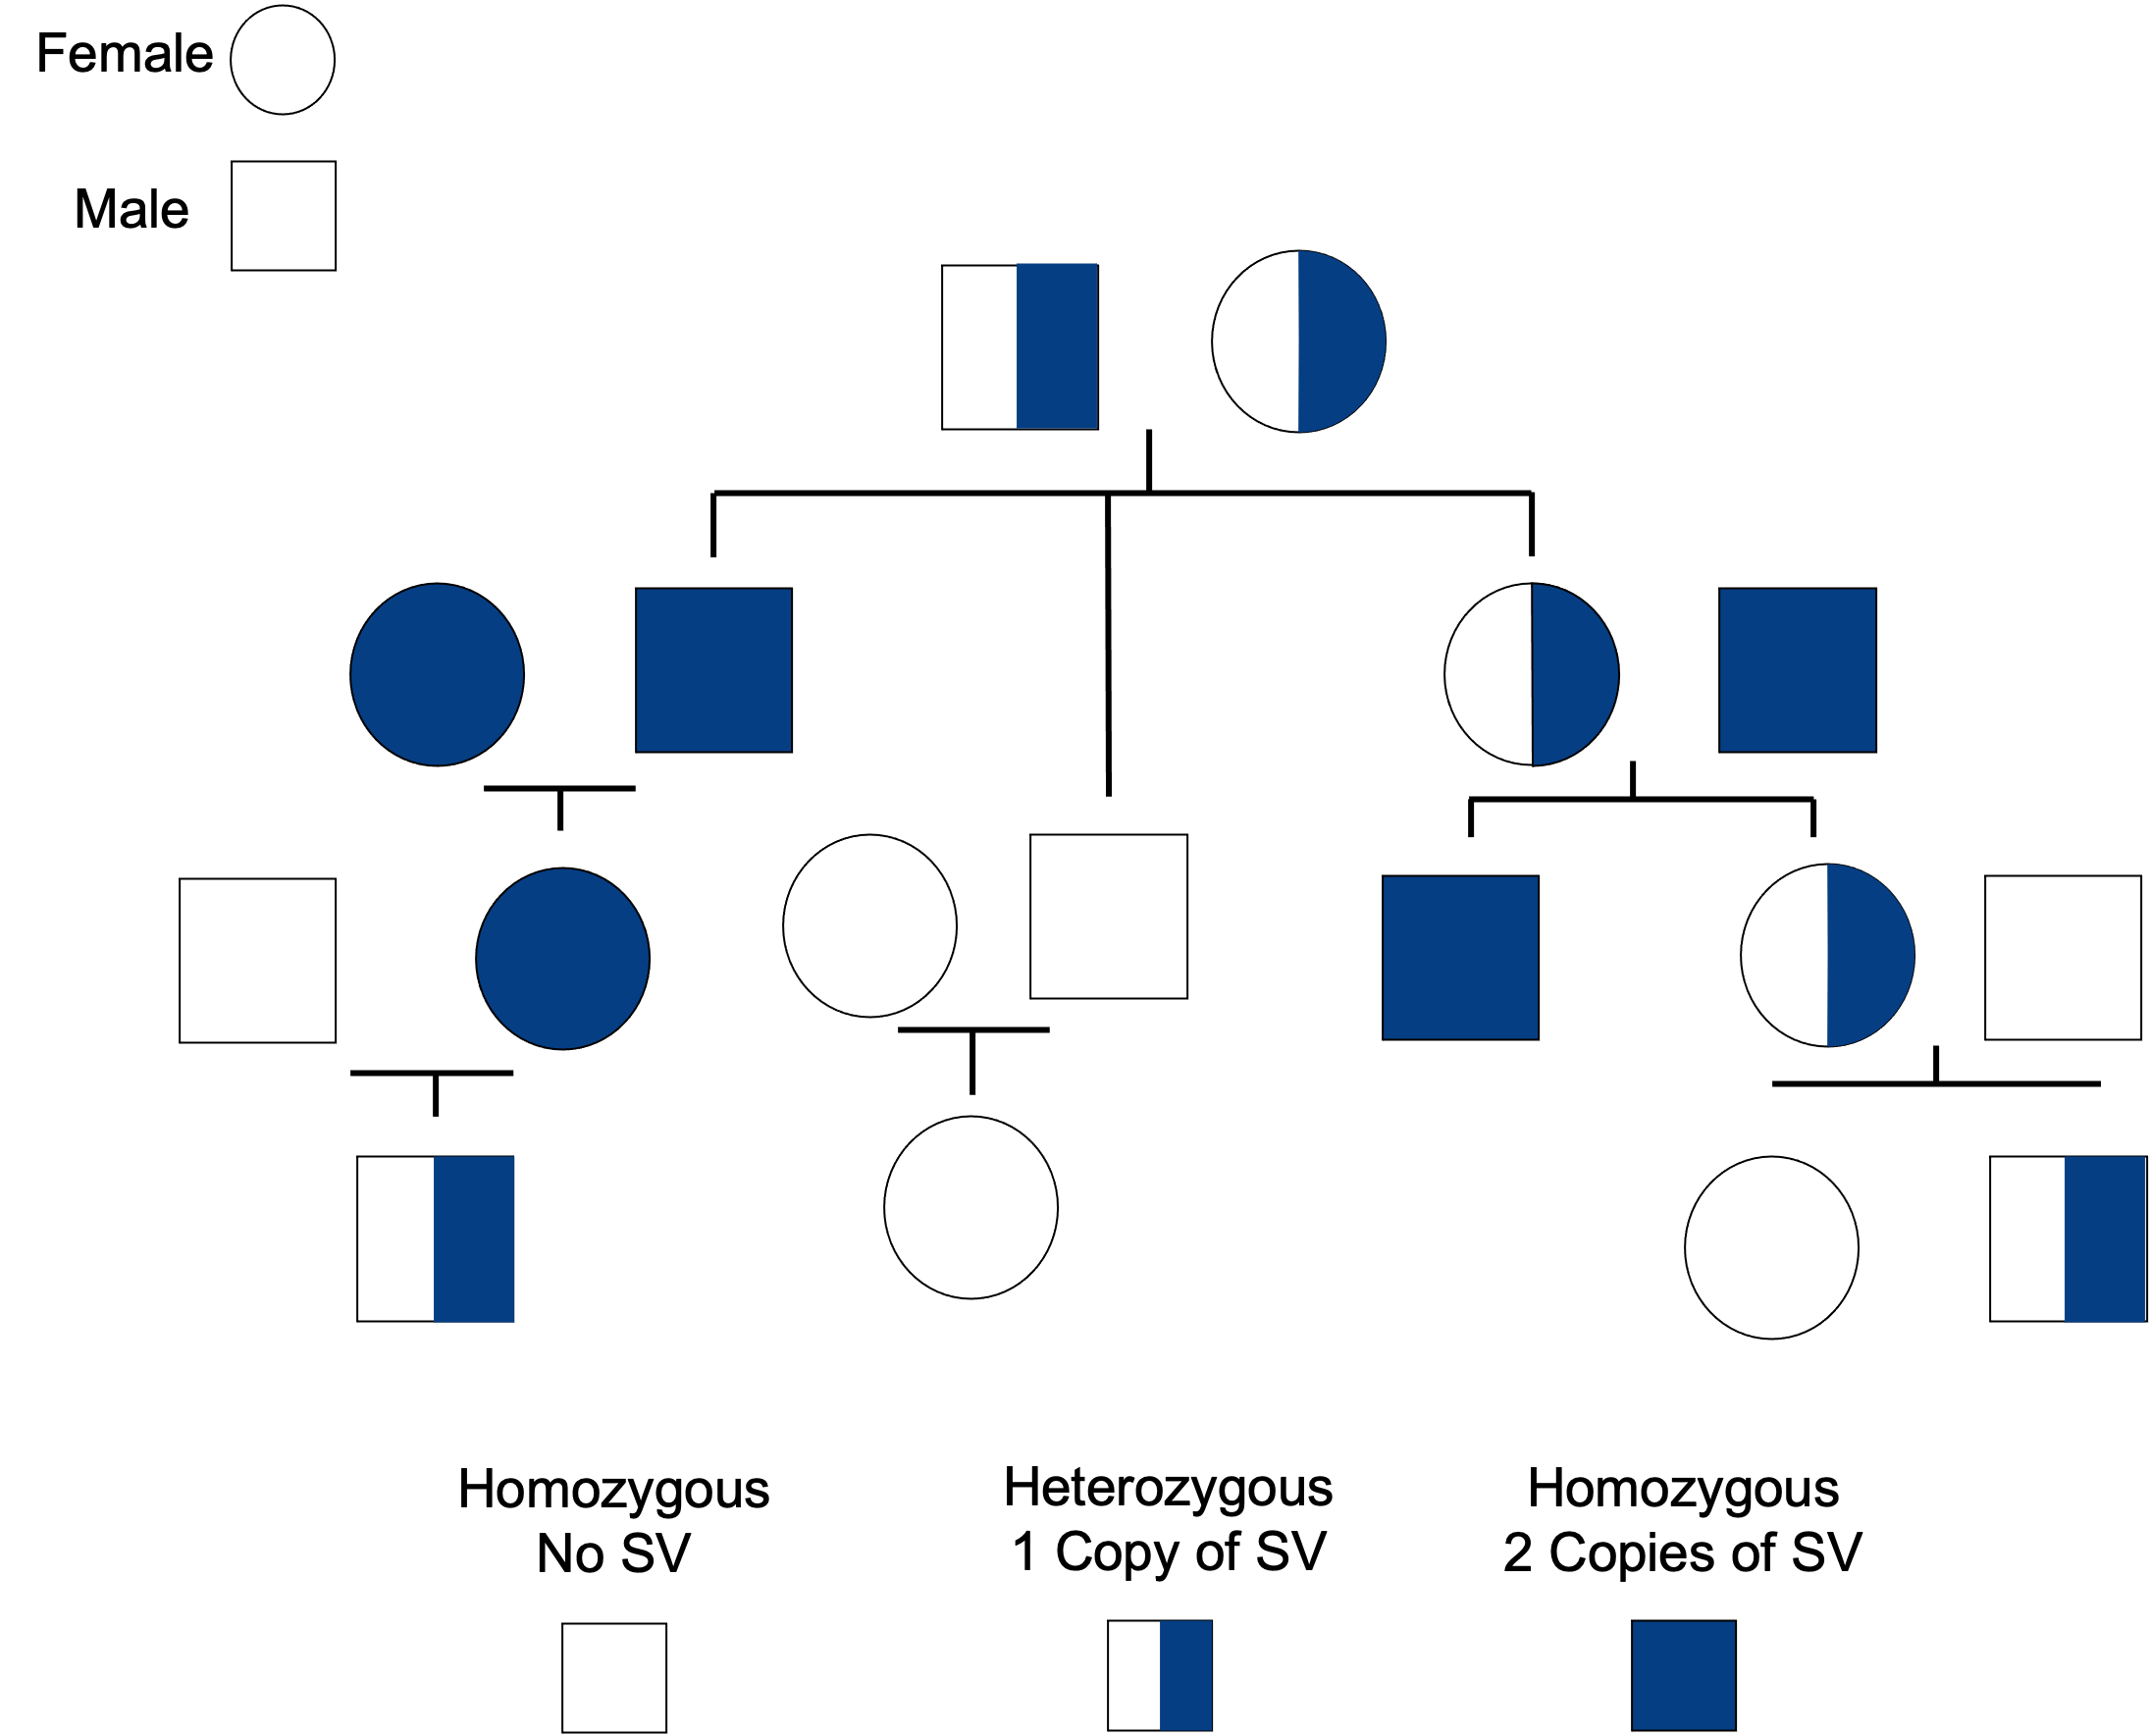
\includegraphics[width=6.0cm]{figs/familial_pedigree.png}}
						%  \vspace{2.0cm}
					\end{minipage}
%				%
%				\begin{minipage}[b]{.48\linewidth}
%						\centering
%						\centerline{\includegraphics[width=4.0cm]{image3}}
%						%  \vspace{1.5cm}
%						\centerline{(b) Results 3}\medskip
%					\end{minipage}
%				\hfill
%				\begin{minipage}[b]{0.48\linewidth}
%						\centering
%						\centerline{\includegraphics[width=4.0cm]{image4}}
%						%  \vspace{1.5cm}
%						\centerline{(c) Result 4}\medskip
%					\end{minipage}
%				%
				\caption{Example of placing a figure with experimental results.}
				\label{fig:res}
				%
			\end{figure}
	\section{METHODS}
	\label{sec:methods}
	
%	All printed material, including text, illustrations, and charts, must be kept
%	within a print area of 7 inches (178 mm) wide by 9 inches (229 mm) high. Do
%	not write or print anything outside the print area. The top margin must be 1
%	inch (25 mm), except for the title page, and the left margin must be 0.75 inch
%	(19 mm).  All {\it text} must be in a two-column format. Columns are to be 3.39
%	inches (86 mm) wide, with a 0.24 inch (6 mm) space between them. Text must be
%	fully justified.
	Here, we describe mathematically our computational framework for predicting SVs for related individuals. More specifically, this study only considers diploid data from one parent (P) and one child (C) for mathematical and computational simplicity. We assume that each signal consists of $n$ candidate locations in the genome where an SV may be present. Further, we separate the signal from the child to consider both inherited and novel SVs individually. For this, we denote the true signal of the parent as $ \fP  \in \{0,1,2\}^n $, and the true signal of the child as $\fC = \fH +\fN \in \{0,1,2\}^{n}$, where $\fH \in \{0,1,2\}^n$ and $\fN \in \{0,1,2\}^n$ correspond to the vectors of inherited ($H$) and novel ($N$) structural variants in the child, respectively.
	
	
	%-------------------------------------------------------------------
	%                    OBSERVATIONAL MODEL
	%-------------------------------------------------------------------
	\subsection{Observational Model}
	We will denote the observation vectors for the parent and the child by the vectors $\sP \in \R^n$, $\sC \in \R^n$, respectively. We assume the data follows a negative binomial distribution:
	\begin{equation} \label{observational_model}
		\begin{bmatrix}
			\sP \\
			\sC
		\end{bmatrix}
		\sim \text{NegBin}
		\Bigg( \begin{bmatrix}
			\zP (2 \lambda_P - \varepsilon) + \yP (\lambda_P - \varepsilon) \\
			\zH (2 \lambda_C - \varepsilon) + \yH (\lambda_C - \varepsilon) + \zN (2 \lambda_C - \varepsilon) + \yN (\lambda_C - \varepsilon) \\
		\end{bmatrix} \Bigg)
	\end{equation}
	
	where $\lambda_P, \lambda_C$ represent the sequencing coverage \textemdash the average number of reads that align to known reference bases\textemdash of the parent and the child, respectively  and $\varepsilon >0$ is used to reflect the measurement errors incurred through the sequencing and mapping processes \cite{MB_diploidTrios, lazar_2021}. \\
	Let 
	$$
	\vec{s} = \begin{bmatrix}
		\sP \\ \sC % \\ \sN
	\end{bmatrix}, \quad 
	\vec{z} = \begin{bmatrix}
		\zP \\ \zH \\ \zN
	\end{bmatrix}, \quad 
	\vec{y} = \begin{bmatrix}
		\yP \\ \yH \\ \yN
	\end{bmatrix}, \quad  
	\vec{f} = \begin{bmatrix}
		\vec{z} \\ \vec{y}
	\end{bmatrix}, 
	$$
	where $\vec{f} \in \{0,1\}^{6n}$. Then we can express the general observation model as
	$$ \vec{s} \sim \text{NegBin}(A \vec{f} + \varepsilon \mathbf{1)}$$
	where $\mathbf{1} \in \R^{2n}$ is the vector of ones, $A$ is the sequence coverage matrix. 
	
	Let $I_n \in \R^{n \times n}$ be the $n \times n$ identity matrix. Then we can write the sequence coverage matrix $A = [A_1 \; A_2] \in \R^{2n \times 6n}$ with
	\renewcommand{\arraystretch}{2}
	\begin{center}
		$$ A_1 = 
		\left[
		\begin{array}{c|c|c}
			(2 \lambda_P - \varepsilon)I_n  & 0 & 0 \\ \hline
			0  & (2 \lambda_C - \varepsilon)I_n &  (2 \lambda_C - \varepsilon)I_n 
		\end{array}
		\right]
		$$
	\end{center}
	and 
	\begin{center}
		$$ A_2 = 
		\left[
		\begin{array}{c|c|c}
			(\lambda_P - \varepsilon)I_n  & 0 & 0 \\ \hline
			0  & (\lambda_C - \varepsilon)I_n &  (\lambda_C- \varepsilon)I_n 
		\end{array}
		\right]
		$$
	\end{center}

%-------------------------------------------------------------------
%                    PROBLEM FORMULATION
%-------------------------------------------------------------------
\subsection{Problem Formulation}
We will assume a Negative Binomial process to model the noise in the sequencing and mapping measurements. The negative binomial distribution can be parameterized in terms of its mean $\vec{\mu}_l = e_{l}^{T} A \vec{f}$ and standard deviation $\vec{\sigma}_{l}^{\,2} = (e_{l}^{T} A \vec{f})_{l} + \frac{1}{r} (e_{l}^{T} A \vec{f})_{l}^{2} $, $l=1, \dots, 2n$, where $e_l$ represents the canonical standard basis vectors. Note that we drop the arrow in the standard basis vectors for ease of notation. We consider the model with the dispersion parameter set to $r =1$ since the standard deviation is maximized with this choice of $r$. With these considerations, the probability of observing the observation vector $\vec{s}$ given the true signal $\vec{f}$, is given by 
\begin{equation} \label{negBinModel_probability}
	p(\vec{s} \; | A\vec{f})\; = \prod_{l=1}^{2n} \left( \frac{1}{1+ (A \vec{f})_l + \varepsilon} \right) \left(  \frac{((A \vec{f})_l + \varepsilon)}{1+ (A \vec{f})_l + \varepsilon} \right)^{s_l} 
\end{equation}
Here, again,  $\varepsilon>0$ is reflective of the sequencing and mapping errors. \\

The solution space for inferring $\vec{f}$ from $\vec{s}$ is exponentially large for large $n$. Thus, we apply a continuous relaxation  of $\vec{f}$ such that its elements lie between $0$ and $1$, i.e. $\mathbf{0} \leq \vec{f} \leq \mathbf{1}$, or equivalently,
\begin{equation}
	\mathbf{0} \leq \, \vec{z}_i, \vec{y}_i \, \leq \mathbf{1}, \quad i \in \{P,H,N\}.
\end{equation}
For the ease of notation, we assume the inequalities read element-wise and denote the vector of all zeros by $\mathbf{0}$ and the vector of all ones by $\mathbf{1}$. \\

The continuous relaxation of our problem formulation allows us to apply a gradient-based maximum likelihood approach to recover the indicator values $\vec{z}_i$ and $\vec{y}_i$ by estimating $A \vec{f}$ such that the probability of observing the vector of negative binomial data $\vec{s}$ is maximized under our statistical model. 

In particular, we seek to minimize the corresponding Negative Binomial negative log-likelihood function
\begin{equation} \label{negBin_negativeLogLikehihood}
	F(\vec{f}) \equiv \sum_{l=1}^{2n}  (1 + s_l)\log \big(1+ e_l^T A \vec{f} + \varepsilon \big) - s_l \log \big( e_l^T A \vec{f} + \varepsilon \big)
\end{equation}

%-------------------------------------------------------------------
%                    FAMILIAL CONSTRAINTS
%-------------------------------------------------------------------
\subsubsection*{Familial Constraints}
We incorporate additional constraints to leverage biological information about $\vec{f}$ to improve accuracy of the model. Since a structural variant cannot be both homozygous and heterozygous at the same time, we require that 
\begin{equation*}
	\mathbf{0} \leq \, \vec{z}_i + \vec{y}_i \, \leq \mathbf{1}, \quad i \in \{P,H,N\}.
\end{equation*}
Recall the signal of the child is comprised of both inherited and novel structural variants, $\fC = \zH + \yH + \zN + \yN$, where a structural variant cannot be both inherited and novel simultaneously. 
\begin{equation*}
	\mathbf{0} \leq \, \zH + \yH + \zN + \yN \, \leq \mathbf{1}.
\end{equation*} 

We consider relatedness in our model. Thus, the child can have an inherited homogeneous SV only if the parent has at least a heterogeneous SV. Similarly, the child can only have an inherited heterogeneous SV if the parent has at least a heterogeneous SV. On the other hand, if the parent has a homogeneous SV at a particular location, then the child must have at least a heterozygous SV at that location, i.e.,
\begin{equation*}
	\mathbf{0} \leq \, \zH   \, \leq \, \zP + \yP  \, \leq \mathbf{1}
\end{equation*}
% \begin{equation*}
	%     \mathbf{0} \leq \, \yH   \, \leq \, \zP + \yP  \, \leq \mathbf{1}
	% \end{equation*}
\begin{equation*}
	\mathbf{0} \leq \, \zP   \, \leq \, \zH + \yH  \, \leq \mathbf{1}
\end{equation*}
Finally, we note that novel structural variants cannot be passed on from the parent. Thus, for a location $j$, if $(\zN)_j + (\yN)_j =1$, then  $(\zP)_j + (\yP)_j =0$. Similarly, if $(\zP)_j + (\yP)_j  =1$, then  $(\zN)_j + (\yN)_j =0$,
\begin{equation*}
	\mathbf{0} \leq \, \zN + \yN   \, \leq \, 1- (\zP +\yP)  \, \leq \mathbf{1}
\end{equation*}
We will denote the set of all vectors satisfying these constraints by $\mathcal{S}$,
% \begin{equation*}
	%      \mathcal{S} =
	%         \begin{Bmatrix*}[l]
		%         &\mathbf{0} \leq \, \vec{z}_i + \vec{y}_i \, \leq \mathbf{1}\\
		%         & \mathbf{0} \leq \, \zH + \yH + \zN + \yN \, \leq \mathbf{1}\\
		%         \vec{f} = [\vec{z}; \vec{y}] \in \R^{6n}: &\mathbf{0} \leq \, \zH   \, \leq \, \zP + \yP  \, \leq \mathbf{1}\\
		%         &\mathbf{0} \leq \, \zH   \, \leq \, \zP + \yP  \, \leq \mathbf{1}\\
		%         &\mathbf{0} \leq \, \zP   \, \leq \, \zH + \yH  \, \leq \mathbf{1}\\
		%         &\mathbf{0} \leq \, \zN + \yN   \, \leq \, 1- (\zP +\yP)  \, \leq \mathbf{1}
		%         \end{Bmatrix*}
	% \end{equation*}
\renewcommand{\arraystretch}{1.3}
\begin{align*}
	\mathcal{S} = \left\{
	\vec{f} = 
	\begin{bmatrix}
		\zP \\ \zH \\ \zN \\ \yP \\ \yH \\ \yN 
	\end{bmatrix} \in \R^{6n} : 
	\begin{matrix*}[l]
		&\mathbf{0} \leq \, \vec{z}_i + \vec{y}_i \, \leq \mathbf{1}\\
		& \mathbf{0} \leq \, \zH + \yH + \zN + \yN \, \leq \mathbf{1}\\
		&\mathbf{0} \leq \, \zH   \, \leq \, \zP + \yP  \, \leq \mathbf{1}\\
		&\mathbf{0} \leq \, \zP   \, \leq \, \zH + \yH  \, \leq \mathbf{1}\\
		&\mathbf{0} \leq \, \zN + \yN   \, \leq \, 1- (\zP +\yP)  \, \leq \mathbf{1}
	\end{matrix*}
	\right\}
\end{align*}. 

%-------------------------------------------------------------------
%                    OPTIMIZATION FORMULATION
%-------------------------------------------------------------------
\subsection{Optimization Formulation}
Structural variants are rare in an individual's genome. Thus, a common challenge with SV recovery is predicting false positive SVs by mistaking fragments that are incorrectly mapped against the reference genome \cite{MB_diploidTrios}. To model this biological reality, we incorporate an $\ell_1$-norm penalty in our objective function to enforce sparsity in our predictions. Further, we assume novel SVs are even more rare since they are not inherited from a parent. Specifically, we use two penalty terms: one for the parent SVs, $\fP$, and the child's inherited SVs, $\fH$, and another penalty term for the child's novel SVs, $\fN$. We define the penalty as follows:

\begin{equation*}
	\text{pen}(\vec{f}) = (\|\zP\|_1 + \|\zH\|_1 + \|\yP\|_1 + \|\yH\|_1) + \gamma (\|\zN\|_1 + \|\yN\|_1)
\end{equation*}
where $\gamma \gg 1$ is the penalty term that enforces greater sparsity in the child's novel SVs. \\

\noindent Our objective function then takes the following form:

\begin{equation} \label{minimizationProblem}
	\begin{aligned}
		& \underset{\vec{f} \in \R^{6n}}{\text{minimize}}
		& & F(\vec{f}) + \tau \text{pen}(\vec{f}) \\
		& \text{subject to}
		& & \vec{f} \in \mathcal{S}
	\end{aligned}
\end{equation}
where $F(\vec{f})$ is the Negative Binomial negative log-likelihood function shown in (\ref{negBin_negativeLogLikehihood}) and $\tau > 0 $ is a regularization parameter. Our approach in solving the minimization problem (\ref{minimizationProblem}) employs sequential quadratic approximations to the Negative Binomial negative log-likelihood $F(\vec{f})$. More specifically, at iteration $k$, we compute a separable quadratic approximation to $F(\vec{f})$ using its second-order Taylor series approximation at $\vec{f}^k$ and approximate the Hessian matrix by a scalar multiple of the identity matrix, $\alpha_k I$ \cite{Marcia_SPIRALTAP}. This quadratic approximation is then defined as

%% Taylor series approximation
\begin{equation*}
	F^k (\vec{f}) \equiv F(\vec{f}^k) + (\vec{f} - \vec{f}^k)^T \nabla F(\vec{f}^k) + \frac{\alpha_k}{2} \|\vec{f} - \vec{f}^k\|_2^2
\end{equation*}
which we use as a surrogate function for $F(\vec{f})$ in (\ref{minimizationProblem}). Using this approximation, the next iterate is given by 

\begin{equation} \label{iterateOG}
	\vec{f}^{k+1} = 
	\begin{aligned}
		& \underset{\vec{f} \in \R^{6n}}{\text{arg min}}
		& & F^k(\vec{f}) + \tau \text{pen}(\vec{f}) \\
		& \text{subject to}
		& & \vec{f} \in \mathcal{S}
	\end{aligned}
\end{equation}
We can reformulate the constrained quadratic subproblem (\ref{iterateOG}) into the following equivalent sequence of subproblems (see \cite{Marcia_SPIRALTAP}):
\begin{equation} \label{subproblemIterate}
	\vec{f}^{k+1} = 
	\begin{aligned}
		& \underset{\vec{f} \in \R^{6n}}{\text{arg min}}
		& & \mathcal{Q}(\vec{f})= \frac{1}{2}\|\vec{f} - \vec{r}^{\,k}\|_2^2 + \frac{\tau}{\alpha_k} \text{pen}(\vec{f}) \\
		& \text{subject to}
		& & \vec{f} \in \mathcal{S}
	\end{aligned}
\end{equation}
where 
\renewcommand{\arraystretch}{1.4}
\begin{equation*}
	\vec{r}^{\,k} = 
	\begin{bmatrix}
		\vec{r}_{z_P}^{\,k} \\ \vec{r}_{z_H}^{\,k} \\ \vec{r}_{z_N}^{\,k}\\
		\vec{r}_{y_P}^{\,k} \\ \vec{r}_{y_H}^{\,k} \\ \vec{r}_{y_N}^{\,k}
	\end{bmatrix} 
	= \vec{f}^k - \frac{1}{\alpha_k} \nabla F(\vec{f}^k)
\end{equation*}
Our objective function $\mathcal{Q}(\vec{f})$ is separable and decouples into the function
$$ \mathcal{Q}(\vec{f}) = \sum_{j=1}^{n} \mathcal{Q}_j(\zP, \zH, \zN, \yP, \yH, \yN)$$
where 
\begin{align*}
	\mathcal{Q}_j(\zP, \zH, \zN, \yP, \yH, \yN) =& \\
	& \frac{1}{2}\Bigg\{
	((\zP - \vec{r}_{\zP}^{\, k})_j)^2 + 
	((\zH - \vec{r}_{\zH}^{\, k})_j)^2 +
	((\zN - \vec{r}_{\zH}^{\, k})_j)^2 \\ & + 
	((\yP - \vec{r}_{\yP}^{\, k})_j)^2 + 
	((\yH - \vec{r}_{\yH}^{\, k})_j)^2 +
	((\yN - \vec{r}_{\yH}^{\, k})_j)^2 \Bigg\} \\ &+
	\frac{\tau}{\alpha_k} \Big\{ |(\zP)_j| + 
	|(\zH)_j| + \gamma |(\zN)_j| + |(\yP)_j| + 
	|(\yH)_j| + \gamma |(\yN)_j|\Big\}
\end{align*}

Since the bounds that define the region $\mathcal{S}$ are component-wise, then  \ref{subproblemIterate} separates into subproblems of the form

\renewcommand{\arraystretch}{1}
\begin{equation} \label{scalarSubprob}
	\begin{aligned}
		\vec{f}^{k+1} = & \underset{ z_P,z_H,z_N,y_P,y_H,y_N \in \R}{\text{arg min}}
		&  \frac{1}{2} \Big\{
		((\zP - \vec{r}_{\zP}^{\, k})_j)^2 + 
		((\zH - \vec{r}_{\zH}^{\, k})_j)^2 +
		((\zN - \vec{r}_{\zH}^{\, k})_j)^2 \\ & & + 
		((\yP - \vec{r}_{\yP}^{\, k})_j)^2 + 
		((\yH - \vec{r}_{\yH}^{\, k})_j)^2 +
		((\yN - \vec{r}_{\yH}^{\, k})_j)^2 \Big\} \\ & & +
		\frac{\tau}{\alpha_k} \; \Big\{ 
		|(\zP)_j| + |(\zH)_j| + \gamma |(\zN)_j|  +
		|(\yP)_j| + |(\yH)_j| + \gamma |(\yN)_j|\Big\} \\
		& \text{subject to} &  \vec{f} \in S
	\end{aligned}
\end{equation}

where for $i \in \{P,H,N\},\,$ $f_i$ and $r_i$  are scalar components of $\vec{f_i}$ and $\vec{r_i}$, respectively, at the same location.  

Note that \ref{scalarSubprob} has closed form solutions (obtained by completing the square and ignoring constant terms), and thus the constrained minimizer can be easily obtained by projecting the unconstrained solution to the feasible set. 





% Then, the subproblem in (\ref{subproblemIterate}) can be separated into scalar minimization problems. The objective function is separable in $\vec{f}$. Thus, (\ref{subproblemIterate}) decouples into $n$ six-dimensional problems of the form 
% \renewcommand{\arraystretch}{1}
% \begin{equation} %\label{subproblemIterate}
	%     \begin{aligned}
		%         \vec{f}^{k+1} = & \underset{\vec{f} = [z_P;z_H;z_N;y_P;y_H;y_N] \in \R^{6}}{\text{arg min}}
		%         & & \frac{1}{2}\|\vec{f} - r^{k}\|_2^2 + \frac{\tau}{\alpha_k} \text{pen}(\vec{f}) \\
		%         & \text{subject to}
		%         & & \vec{f} \in S
		%     \end{aligned}
	% \end{equation}
% where $r^k = [r^k_{z_P},r^k_{z_H},r^k_{z_N},r^k_{y_P},r^k_{y_H},r^k_{y_N}]^T$ and $f = [z_P,z_H,z_N,y_P,y_H,y_N]^T$ correspond to the components of $\vec{r}^{\,k}$ and $\vec{f}$, respectively, and the set $S$ is similar to the set $\mathcal{S}$ with the distinction that it is restricted to the particular candidate SV position.  

%-------------------------------------------------------------------
%                    OPTIMIZATION APPROACH
%-------------------------------------------------------------------
\subsection{Optimization Approach}
We propose solving our problem using an alternating block-coordinate descent approach, following the methods used in previous work \cite{MB_diploidTrios, lazar_2021,MB_SingleParentDiploid}. For this,  we fix all but one individual and solve (\ref{subproblemIterate}) over both indicator variables for that individual. We continue successively minimizing both indicator variables for each individual while the other individuals are fixed. The feasible region for this step is illustrated in \ref{label}\\
	\begin{figure*}[h]
	\begin{minipage}[h]{0.30\linewidth}
		\centering
		\centerline{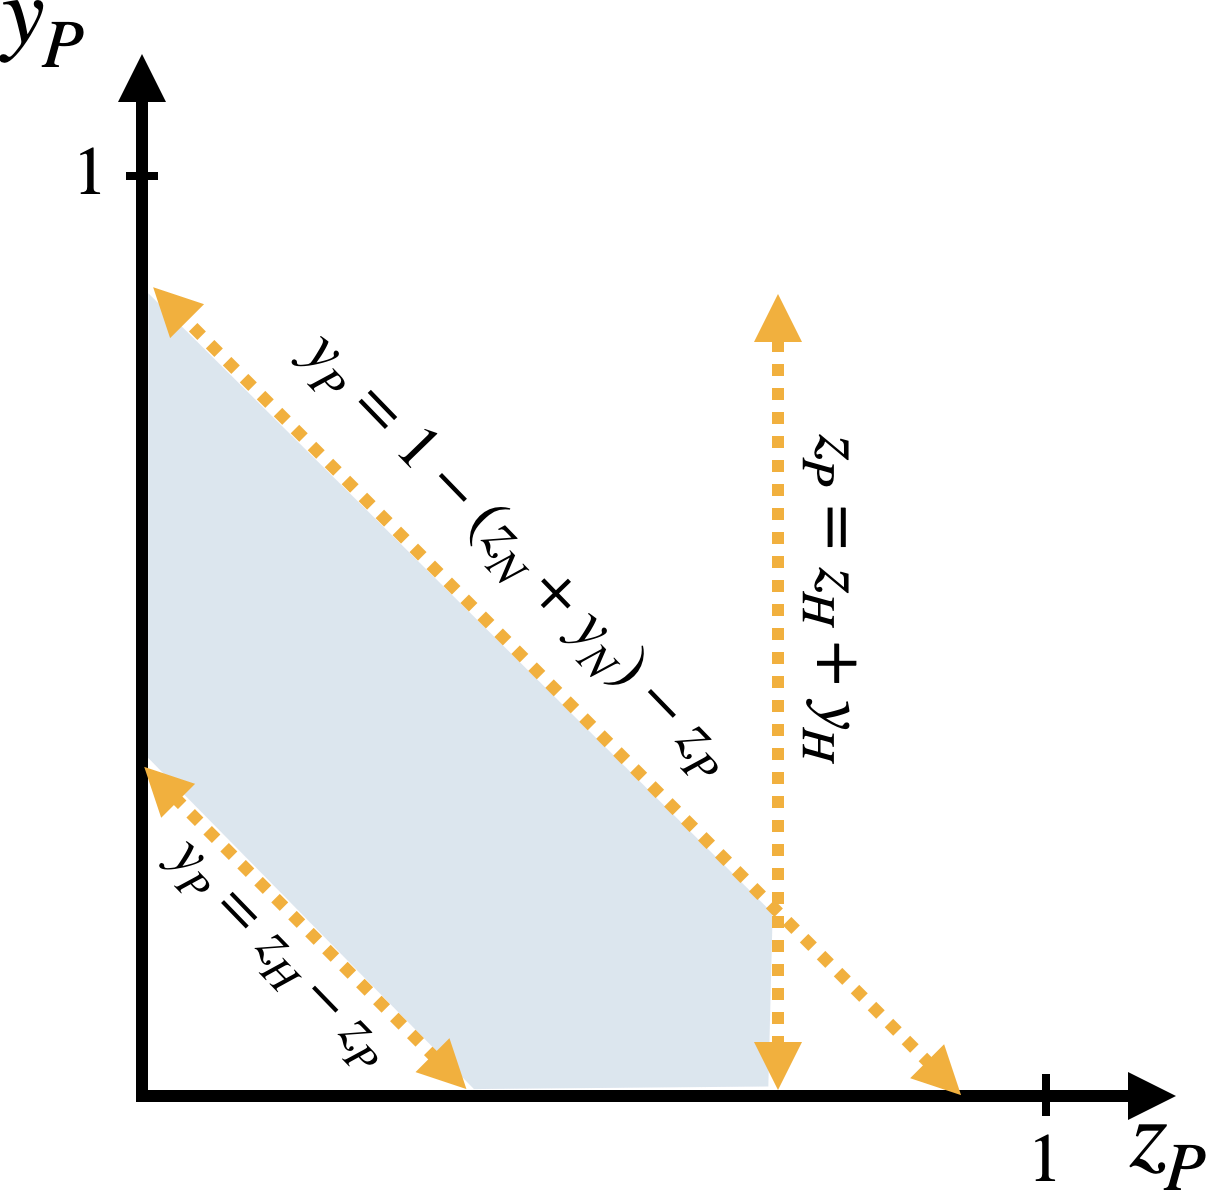
\includegraphics[width=4.0cm]{figs/parent_region.png}}
		\centerline{(a) Results 3}\medskip
		%  \vspace{2.0cm}
	\end{minipage}
					%
					\begin{minipage}[h]{.30\linewidth}
								\centering
								\centerline{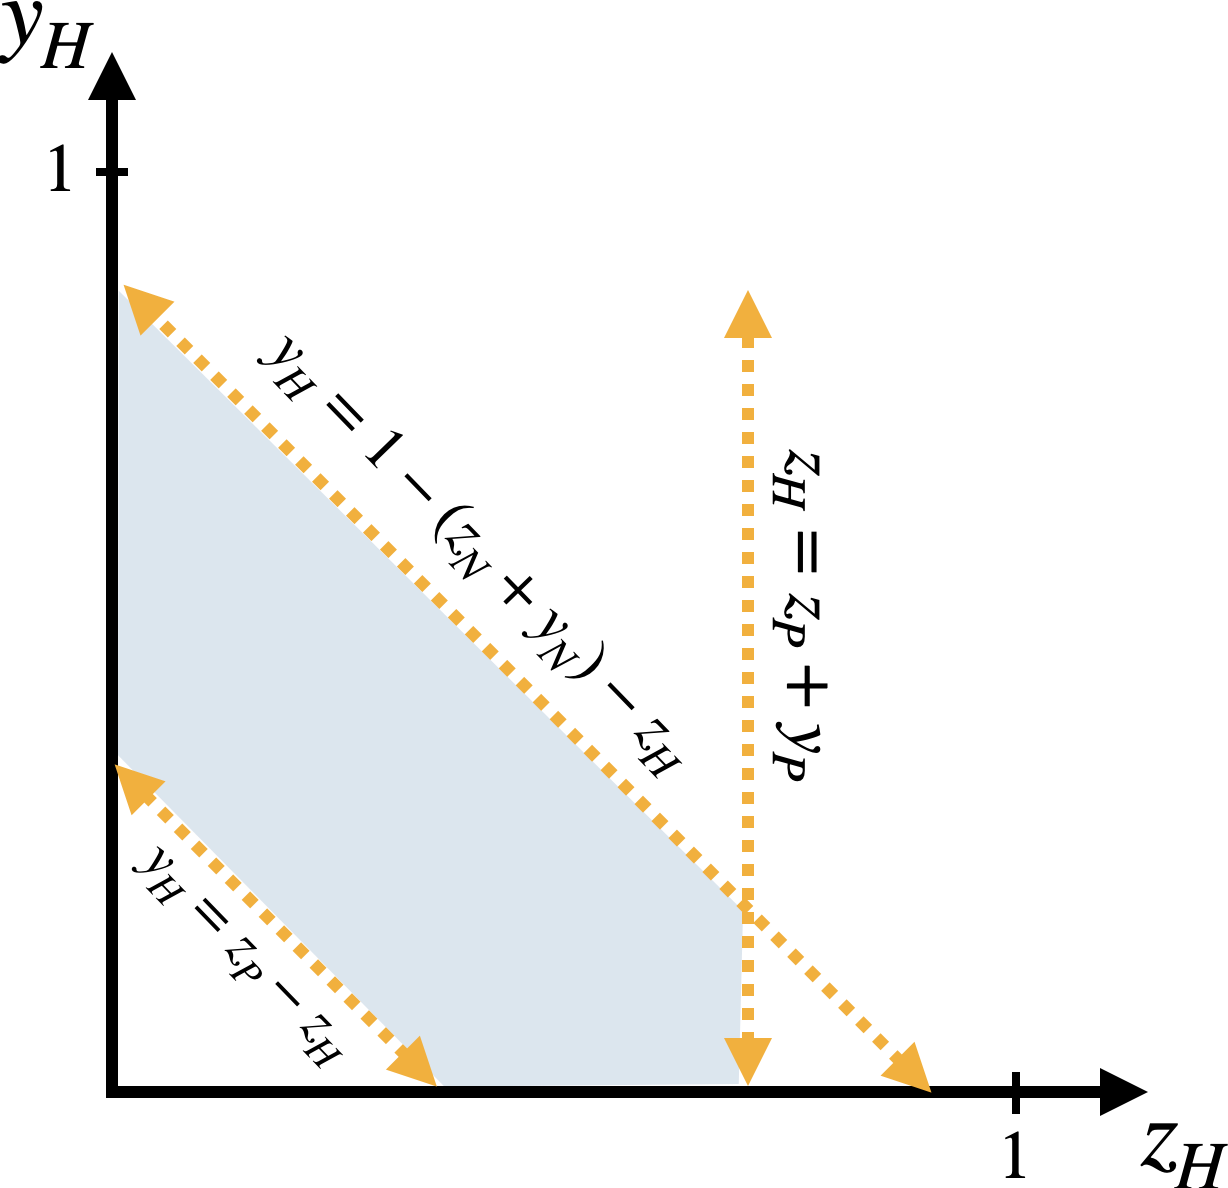
\includegraphics[width=4.0cm]{figs/inherited_region.png}}
								%  \vspace{1.5cm}
								\centerline{(b) Results 3}\medskip
							\end{minipage}
				%	\hfill
					\begin{minipage}[h]{0.30\linewidth}
								\centering
								\centerline{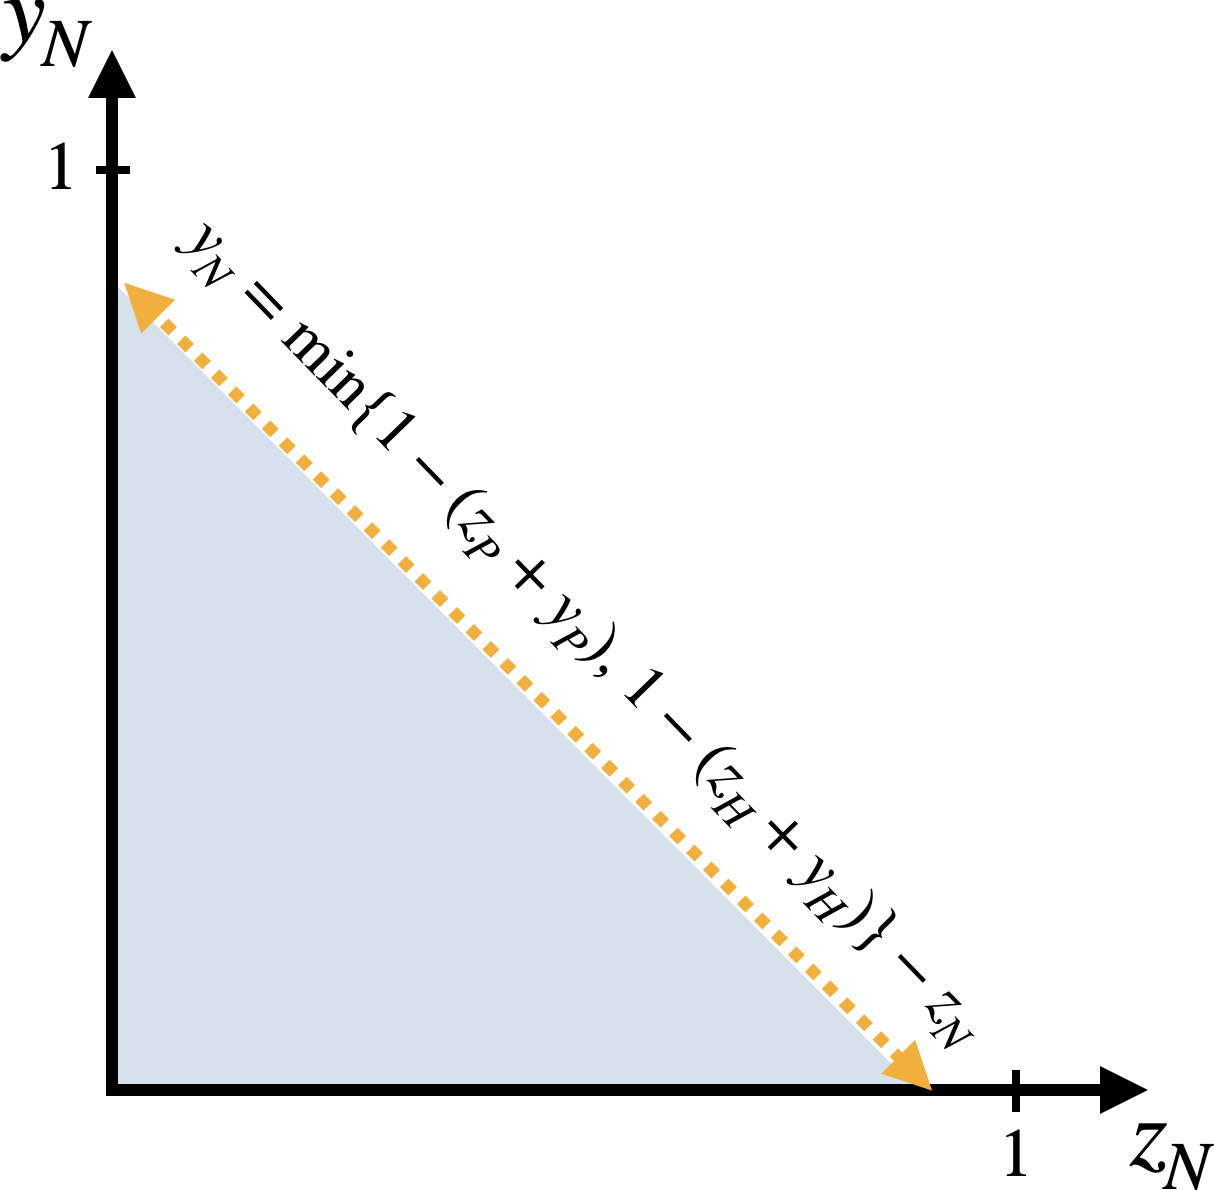
\includegraphics[width=4.0cm]{figs/novel_region.png}}
								%  \vspace{1.5cm}
								\centerline{(c) Result 4}\medskip
							\end{minipage}
					%
	\caption{Example of placing a figure with experimental results.}
	\label{fig:regions}
	%
\end{figure*}

\noindent \textbf{Step 0:} We begin by computing the unconstrained minimizer of (\ref{subproblemIterate}), which is given by $\vec{f} = \vec{r}^{\,k} - \frac{\tau}{\alpha_k}\gamma\mathbf{1}$. % not this. it is something like 1/alpha[tau; tau; tau*gamma; tau; tau; tau*gammas]
Next,  we initialize the child's inherited and novel indicator variables by applying the following rule:
\begin{equation*}
	\begin{aligned}
		\hat{z}_H^{(0)} = \{0,r_{z_H}^k - \frac{\tau}{\alpha_k},1 \}, & \quad \hat{z}_N^{(0)} = \{0,r_{z_N}^k - \frac{\tau}{\alpha_k}\gamma,1 \},\\
		\hat{y}_H^{(0)} = \{0,r_{y_H}^k - \frac{\tau}{\alpha_k},1 \}, &
		\quad \hat{y}_N^{(0)} = \{0,r_{y_N}^k - \frac{\tau}{\alpha_k}\gamma,1 \}
	\end{aligned}
\end{equation*}
Further, if $\hat{z}_H^{(0)} + \hat{y}_H^{(0)}>1$, then we let $\hat{z}_H^{(0)} = \hat{y}_H^{(0)} = 0.5$. We adjust $\hat{z}_N^{(0)}$ and $\hat{y}_N^{(0)}$ similarly. We apply these rules to ensure our initialization is consistent with the set of feasible solutions. To initialize the parent indicator variables, we let $\hat{z}_P^{(0)} = r_{z_P}^k - \frac{\tau}{\alpha_k}$ and $\hat{y}_P^{(0)} = r_{y_P}^k - \frac{\tau}{\alpha_k}$. 
We initialize the index with $i=1$. \\

\noindent \textbf{Step 1:} Once we have obtained estimates for child's inherited and novel diploid indicator variables, $\hat{z}_H^{(i-1)}, \hat{y}_H^{(i-1)}, \hat{z}_N^{(i-1)}, \hat{y}_N^{(i-1)}$, from the previous iteration, we project $\hat{z}_P^{(i-1)}$ and $\hat{y}_P^{(i-1)}$ onto the feasible set $S$ with fixed inherited and novel variables to obtain the new parent indicator values $\hat{z}_P^{(i)}$ and $\hat{y}_P^{(i)}$. This projection is similar to the projections done in \cite{MB_SingleParentDiploid, MB_diploidTrios}. \\

\noindent \textbf{Step 2:} After obtaining the new estimates for the parent diploid indicator variables $\hat{z}_P^{(i)}$ and $\hat{y}_P^{(i)}$ from Step 1, we project $\hat{z}_H^{(i-1)}, \hat{y}_H^{(i-1)}$ onto our feasible set $S$ with fixed parent and child's novel indicator variables to obtain the new child's inherited indicator variables $\hat{z}_H^{(i)}$ and $\hat{y}_H^{(i)}$.\\ 

\noindent \textbf{Step 3:} After obtaining the new estimates for the child's inherited diploid indicator variables $\hat{z}_H^{(i)}$ and $\hat{y}_H^{(i)}$ from Step 2, we project $\hat{z}_N^{(i-1)}, \hat{y}_N^{(i-1)}$ onto our feasible set $S$ with fixed parent and child's inherited indicator variables to obtain the new child's novel indicator variables $\hat{z}_N^{(i)}$ and $\hat{y}_N^{(i)}$. \\

We repeat Steps 1, 2, and 3 until some convergence criteria are satisfied. Steps 1 and 2  result in identical feasible regions. 

%-------------------------------------------------------------------
%                    RESULTS
%-------------------------------------------------------------------
\section{Results}
In order to evaluate the effectiveness of our proposed method, we implemented it in MATLAB by modifying the existing SPIRAL approach \cite{Marcia_SPIRALTAP} to include the negative binomial statistical method \cite{Marcia_SPIRALTAP} to solve the quadratic subproblems. We refer to the new algorithm as NEgative Binomial optimization Using $\ell_1$ penalty Algorithm (NEBULA). We compare SPIRAL and NEBULA. We compared the Poisson-based predictions with the Negative Binomial-based predictions in Sec.\ref{subsec:simulated_data}. The regularization parameters ($\tau, \gamma$) were chosen to obtain the maximum area under the curve (AUC) for the receiver operating characteristic (ROC). The algorithm terminates if the relative difference between consecutive iterates converged to $\|\vec{f}^{k+1} - \vec{f}^{k}\|/\|\vec{f}^{k}\| \leq 10^{-8}$.

\subsection{Simulated Data}
\label{subsec:simulated_data}
Similar to previous approaches, we simulated two parent signals of size $10^5$ with a set number of structural variants and a set similarity of $80\%$ between the parent signals \cite{MB_diploidTrios, MB_SingleParentDiploid}. In the parent signals, $5000$ locations were chosen at random to be structural variants. We then constructed the child signal by first applying a logical implementation of inheritance to $\lfloor 5000p \rfloor$ randomly selected parent structural variants (where $p$ is the percent overlap between parent and child SVs). Next, we chose  $(5000 - \lfloor 5000p \rfloor)$ locations from the remaining $(10^5 - 5000)$ that were not chosen as a parent variant to be novel variants in the child.  After forming the true signals for each individual, the observed signals were generated by sampling from the Negative Binomial distribution with a given coverage and error.For the purpose of testing the proposed approach, only one parent signal was used. The data simulation code was implemented in Python. \\\\
%Specifically, we used a logical implementation of inheritance (e.g. if both parents were homozygous for a variant, then the child would also be homozygous and so on) with a parent similarity of $80\%$.
\textbf{Analysis.} Given an optimal $\tau, \gamma$ values, our method is better able to reconstruct the homozygous signals for each individual despite large sequencing and mapping error, $\varepsilon = 0.5$. In Figure \textcolor{red}{INSERT HERE} we show both Receiving Operating Characteristic (ROC) and Precision-Recall (PR) curves obtained for a simulated data set where the parents share $80\%$ of their SVs. Similar to previous work, we use the area under the curve (AUC) for the ROC curves to measure the ability of SPIRAL and NEBULA to distinguish between classes. % say something about NEBULA showing improvements to SPIRAL
Since SVs are very rare and we are faced with strongly imbalanced data, however, we incorporate Precision-Recall curves to gain a deeper understanding of the performance of our algorithm as it relates to false positives. We see improvements in area under the curve and average precision for the parent and child's inherited signals. We also see comparable performance for the reconstruction of the child's novel signal.

	\begin{figure}[htb]
			
			\begin{minipage}[b]{1.0\linewidth}
					\centering
					\centerline{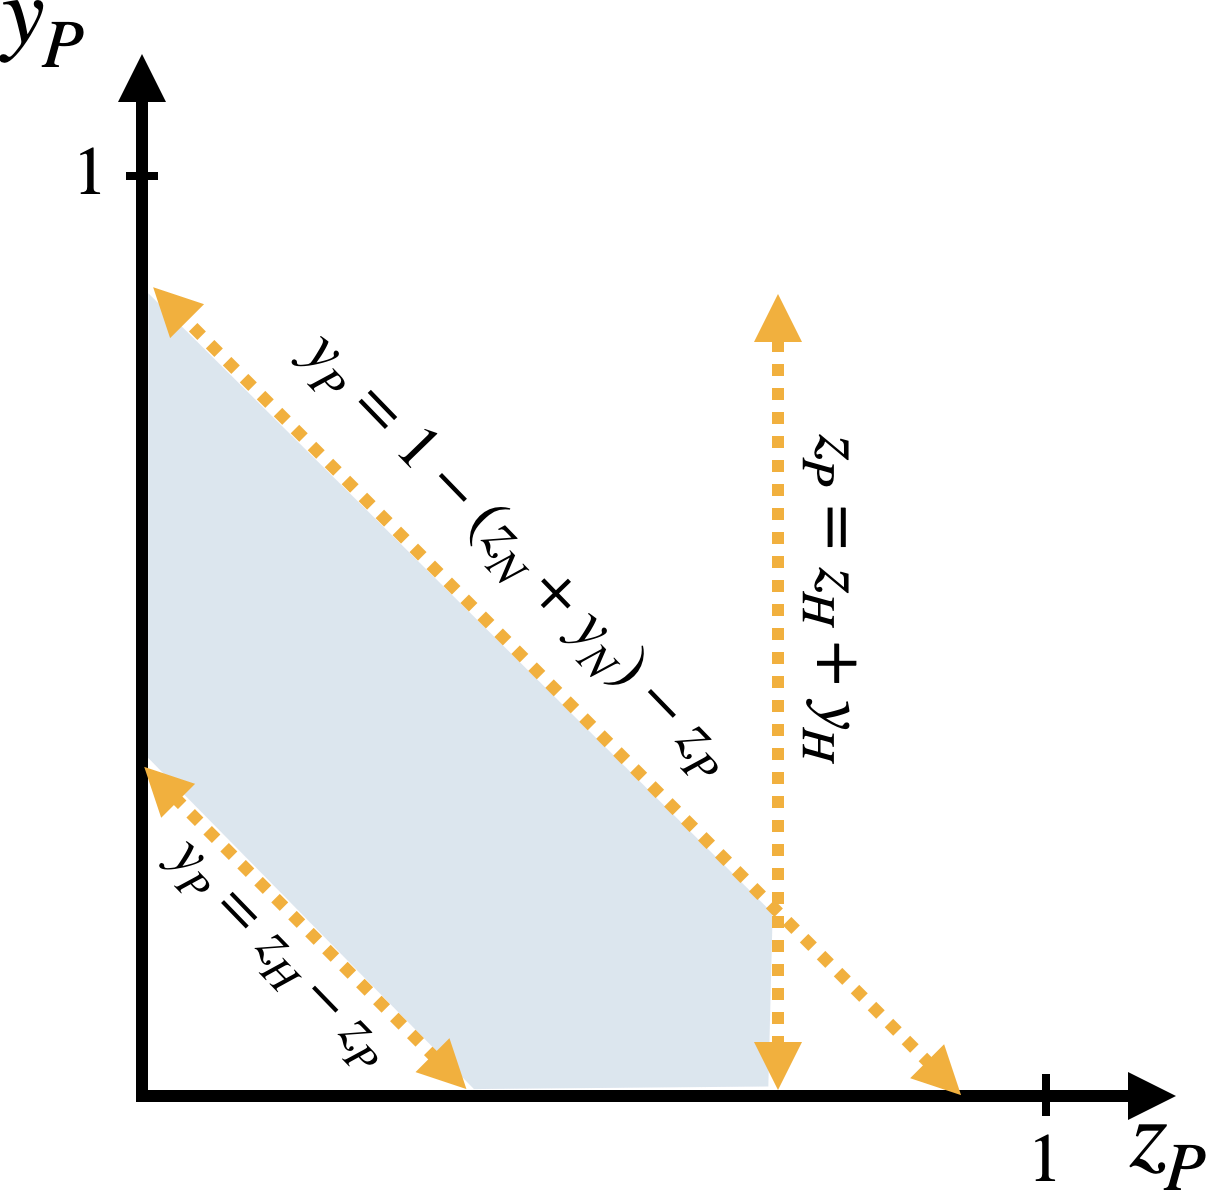
\includegraphics[width=4.0cm]{figs/parent_region.png}}
					%  \vspace{2.0cm}
					\centerline{(a) Result 1}\medskip
				\end{minipage}
			%
			\begin{minipage}[b]{.48\linewidth}
					\centering
					\centerline{\includegraphics[width=4.0cm]{image3}}
					%  \vspace{1.5cm}
					\centerline{(b) Results 3}\medskip
				\end{minipage}
			\hfill
			\begin{minipage}[b]{0.48\linewidth}
					\centering
					\centerline{\includegraphics[width=4.0cm]{image4}}
					%  \vspace{1.5cm}
					\centerline{(c) Result 4}\medskip
				\end{minipage}
			%
			\caption{Example of placing a figure with experimental results.}
			\label{fig:res}
			%
		\end{figure}
\section{Conclusion}
We present an optimization method to detect SVs in low-coverage sequencing data from related individuals. This method leverages Mendelian inheritance to improve signal reconstruction of noisy data. This extends previous work that focused on a Poisson-based optimization algorithm. 


In future studies, we intend to apply this work to a two parent and one child framework. 

\textbf{Acknowledgement.} This work was supported by \textcolor{red}{insert here}

%	\section{PAGE TITLE SECTION}
%	\label{sec:pagestyle}
%	
%	The paper title (on the first page) should begin 1.38 inches (35 mm) from the
%	top edge of the page, centered, completely capitalized, and in Times 14-point,
%	boldface type. The authors' name(s) and affiliation(s) appear below the title
%	in capital and lower case letters.  Papers with multiple authors and
%	affiliations may require two or more lines for this information. Please note
%	that papers should not be submitted blind; include the authors' names on the
%	PDF.
%	
%	\section{TYPE-STYLE AND FONTS}
%	\label{sec:typestyle}
%	
%	To achieve the best rendering both in printed proceedings and electronic proceedings, we
%	strongly encourage you to use Times-Roman font.  In addition, this will give
%	the proceedings a more uniform look.  Use a font that is no smaller than nine
%	point type throughout the paper, including figure captions.
%	
%	In nine point type font, capital letters are 2 mm high.  {\bf If you use the
%		smallest point size, there should be no more than 3.2 lines/cm (8 lines/inch)
%		vertically.}  This is a minimum spacing; 2.75 lines/cm (7 lines/inch) will make
%	the paper much more readable.  Larger type sizes require correspondingly larger
%	vertical spacing.  Please do not double-space your paper.  TrueType or
%	Postscript Type 1 fonts are preferred.
%	
%	The first paragraph in each section should not be indented, but all the
%	following paragraphs within the section should be indented as these paragraphs
%	demonstrate.
%	
%	\section{MAJOR HEADINGS}
%	\label{sec:majhead}
%	
%	Major headings, for example, "1. Introduction", should appear in all capital
%	letters, bold face if possible, centered in the column, with one blank line
%	before, and one blank line after. Use a period (".") after the heading number,
%	not a colon.
%	
%	\subsection{Subheadings}
%	\label{ssec:subhead}
%	
%	Subheadings should appear in lower case (initial word capitalized) in
%	boldface.  They should start at the left margin on a separate line.
%	
%	\subsubsection{Sub-subheadings}
%	\label{sssec:subsubhead}
%	
%	Sub-subheadings, as in this paragraph, are discouraged. However, if you
%	must use them, they should appear in lower case (initial word
%	capitalized) and start at the left margin on a separate line, with paragraph
%	text beginning on the following line.  They should be in italics.
%	
%	\section{PRINTING YOUR PAPER}
%	\label{sec:print}
%	
%	Print your properly formatted text on high-quality, 8.5 x 11-inch white printer
%	paper. A4 paper is also acceptable, but please leave the extra 0.5 inch (12 mm)
%	empty at the BOTTOM of the page and follow the top and left margins as
%	specified.  If the last page of your paper is only partially filled, arrange
%	the columns so that they are evenly balanced if possible, rather than having
%	one long column.
%	
%	In LaTeX, to start a new column (but not a new page) and help balance the
%	last-page column lengths, you can use the command ``$\backslash$pagebreak'' as
%	demonstrated on this page (see the LaTeX source below).
%	
%	\section{PAGE NUMBERING}
%	\label{sec:page}
%	
%	Please do {\bf not} paginate your paper.  Page numbers, session numbers, and
%	conference identification will be inserted when the paper is included in the
%	proceedings.
%	
%	\section{ILLUSTRATIONS, GRAPHS, AND PHOTOGRAPHS}
%	\label{sec:illust}
%	
%	Illustrations must appear within the designated margins.  They may span the two
%	columns.  If possible, position illustrations at the top of columns, rather
%	than in the middle or at the bottom.  Caption and number every illustration.
%	All halftone illustrations must be clear black and white prints.  Colors may be
%	used, but they should be selected so as to be readable when printed on a
%	black-only printer.
%	
%	Since there are many ways, often incompatible, of including images (e.g., with
%	experimental results) in a LaTeX document, below is an example of how to do
%	this \cite{Lamp86}.
%	
%	\section{FOOTNOTES}
%	\label{sec:foot}
%	
%	Use footnotes sparingly (or not at all!) and place them at the bottom of the
%	column on the page on which they are referenced. Use Times 9-point type,
%	single-spaced. To help your readers, avoid using footnotes altogether and
%	include necessary peripheral observations in the text (within parentheses, if
%	you prefer, as in this sentence).
%	
%	% Below is an example of how to insert images. Delete the ``\vspace'' line,
%	% uncomment the preceding line ``\centerline...'' and replace ``imageX.ps''
%	% with a suitable PostScript file name.
%	% -------------------------------------------------------------------------
%%	\begin{figure}[htb]
%%		
%%		\begin{minipage}[b]{1.0\linewidth}
%%			\centering
%%			\centerline{\includegraphics[width=8.5cm]{image1}}
%%			%  \vspace{2.0cm}
%%			\centerline{(a) Result 1}\medskip
%%		\end{minipage}
%%		%
%%		\begin{minipage}[b]{.48\linewidth}
%%			\centering
%%			\centerline{\includegraphics[width=4.0cm]{image3}}
%%			%  \vspace{1.5cm}
%%			\centerline{(b) Results 3}\medskip
%%		\end{minipage}
%%		\hfill
%%		\begin{minipage}[b]{0.48\linewidth}
%%			\centering
%%			\centerline{\includegraphics[width=4.0cm]{image4}}
%%			%  \vspace{1.5cm}
%%			\centerline{(c) Result 4}\medskip
%%		\end{minipage}
%%		%
%%		\caption{Example of placing a figure with experimental results.}
%%		\label{fig:res}
%%		%
%%	\end{figure}
%%	
	
	% To start a new column (but not a new page) and help balance the last-page
	% column length use \vfill\pagebreak.
	% -------------------------------------------------------------------------
	%\vfill
	%\pagebreak
	
	\section{COPYRIGHT FORMS}
	\label{sec:copyright}
	
	You must submit your fully completed, signed IEEE electronic copyright release
	form when you submit your paper. We {\bf must} have this form before your paper
	can be published in the proceedings.
	
%	\section{RELATION TO PRIOR WORK}
%	\label{sec:prior}
%	
%	The text of the paper should contain discussions on how the paper's
%	contributions are related to prior work in the field. It is important
%	to put new work in  context, to give credit to foundational work, and
%	to provide details associated with the previous work that have appeared
%	in the literature. This discussion may be a separate, numbered section
%	or it may appear elsewhere in the body of the manuscript, but it must
%	be present.
%	
%	You should differentiate what is new and how your work expands on
%	or takes a different path from the prior studies. An example might
%	read something to the effect: "The work presented here has focused
%	on the formulation of the ABC algorithm, which takes advantage of
%	non-uniform time-frequency domain analysis of data. The work by
%	Smith and Cohen \cite{Lamp86} considers only fixed time-domain analysis and
%	the work by Jones et al \cite{C2} takes a different approach based on
%	fixed frequency partitioning. While the present study is related
%	to recent approaches in time-frequency analysis [3-5], it capitalizes
%	on a new feature space, which was not considered in these earlier
%	studies."
	
	\vfill\pagebreak
	
	\section{REFERENCES}
	\label{sec:refs}
	
%	List and number all bibliographical references at the end of the
%	paper. The references can be numbered in alphabetic order or in
%	order of appearance in the document. When referring to them in
%	the text, type the corresponding reference number in square
%	brackets as shown at the end of this sentence \cite{C2}. An
%	additional final page (the fifth page, in most cases) is
%	allowed, but must contain only references to the prior
%	literature.
	
	% References should be produced using the bibtex program from suitable
	% BiBTeX files (here: strings, refs, manuals). The IEEEbib.bst bibliography
	% style file from IEEE produces unsorted bibliography list.
	% -------------------------------------------------------------------------
	\bibliographystyle{IEEEbib}
	\bibliography{strings,references.bib}
	
\end{document}
